Chapter 10: if we include predictor variable containing two categories into the linear model, then the resulting $b$ for that predictor compares the difference between the mean score for the two categories. 

Chapter 11: says that if we want to include a categorical predictor that contains more than two categories, this can be achieved by recoding that variable into several categorical predictors, each of which has only two categories (dummy coding). When we do this, $b$s for predictors represent differences between means.

Chapter 9: use F-statistics to test the overall fit of linear model, for ANOVA, we can do the same: we can use F to test  whether we significantly predict the outcome variable by using group means. 

For ANOVA, we can use an $F$ to test whether we significantly predict the outcome variable by using group means (which tells us whether overall, the group means are significantly different) and then use the specific model parameters ($b$s) to tell us which means differ from which. 

ANOVA is simply F-statistics which is use as a test of the fit of a linear model, its just that the linear model consists of group means.Learning ANOVA as a linear model framework allows ANOVA to be extended to more complex situations (e.g. multiple predictors, unequal group sizes) without the need to get bogged down in maths.

Another way to learn ANOVA is through use of F-statistics to compare means known as the variance-ratio method. This approach is fine for simple design analysis but is difficult to use in complex situations such as the analysis of covariance.
\clearpage

\subsection{Example}
\begin{figure}[h]
	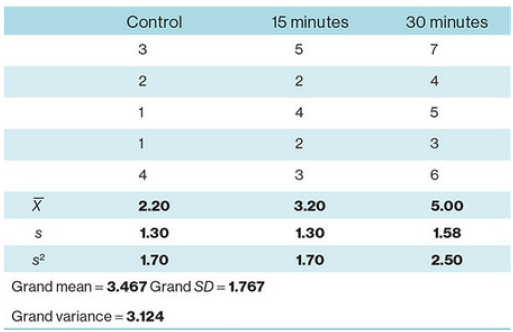
\includegraphics[width=.6\textwidth,height=50mm]{Chapter 12 GLM 1 Comparing Several Independent Means ANOVA/dataexample.PNG}
	\caption{Predicting happiness from exposure to dog therapy of different durations. 3 groups: Control, 15 mins, 30 mins}
\end{figure}

This can be incorporated into a linear model by including 2 dummy variable (each assigned a $b$-value).

When we assign dummy variable, one group must be the base like condition, $b_0$. In dog therapy example, we use the control group as the baseline category as we are interested in comparing both the 15 and 30 minutes groups to the control group. Thus the equation of the model is:

\begin{center}
$\text{Happiness}_i = b_0 + b_1\text{Long}_i + b_2\text{Short}_i + \varepsilon_i$
\end{center}


By rearranging the variables, we can find out get the equation for $\bar{X}_{\text{control}},\bar{X}_{\text{30 mins}},\bar{X}_{\text{15 mins}}$, which are predicted value of happiness for each group. 

\begin{equation}
\begin{split}
\text{Happiness}_i & = b_0 + (b_1 * 0) + (b_2 * 0)   \\
\bar{X}_{\text{control}} & = b_0
\end{split}
\end{equation}

substitute $b_0$, into equation for 30mins:
\begin{equation}
\begin{split}
\text{Happiness}_i & = b_0 + (b_1 * 1) +  (b_2 * 0)   \\
& = b_0 + b_1 \\
\bar{X}_{\text{30 mins}} & = \bar{X}_{\text{control}} + b_1 \\
b_1 & = \bar{X}_{\text{30 mins}} - \bar{X}_{\text{control}} 
\end{split}
\end{equation}

substitute $b_0$, into equation for 15 mins:
\begin{equation}
\begin{split}
\text{Happiness}_i & = b_0 + (b_1 * 0) +  (b_2 * 1)   \\
& = b_0 + b_1 \\
\bar{X}_{\text{15 mins}} & = \bar{X}_{\text{control}} + b_2 \\
b_2& = \bar{X}_{\text{15 mins}} - \bar{X}_{\text{control}} 
\end{split}
\end{equation}

Equation 5.3 shows that the $b$ value for dummy variable representing the 15 minute group is the difference between the means for the 15 minute group and control group.

By coding a new dummy variable for each of the variable, we can use linear regression and F test to test the overall fit of the model.

\section{Logic of F statistics}

F test is an overall test that does not specify differences between specific means. However, the model parameters ($b$ values) do. 

F-statistic tests the overall fit of a linear model to a set of observed data. F is the ratio of how good the model is compared to how bad it is (its error). When model is based on group means, our predictions from the model are the means. If group means are the same, then our ability to predict observed data will be poor (F will be small), bt if the means differ, we will be able to better discriminate between cases from different groups (F will be large). In the dog therapy context, F basically tells us whether the group means are significantly different.

From above we know that $b_1 = \bar{X}_{\text{30 mins}} - \bar{X}_{\text{control}} $  and $b_2 = \bar{X}_{\text{15 mins}} - \bar{X}_{\text{control}} $. However, if null hypothesis is true, and all the groups have the same group mean, then these $b$ coefficients will be 0 (if group means are equal then differences between them will be 0).\\

We can apply same logic as for any linear model:
\begin{itemize}
\item The model that represents ‘no effect’ or ‘no relationship between the predictor 
variable and the outcome’ is one where the predicted value of the outcome is always
the grand mean (the mean of the outcome variable).
\item We can fit a different model to the data that represents our alternative hypotheses.
We compare the fit of this model to the fit of the null model (i.e., using the grand
mean).
\item The intercept and one or more parameters (b) describe the model.
\item The parameters determine the shape of the model that we have fitted; therefore, the
bigger the coefficients, the greater the deviation between the model and the null
model (grand mean).
\item In experimental research the parameters (b) represent the differences between group
means. The bigger the differences between group means, the greater the difference
between the model and the null model (grand mean).
\item If the differences between group means are large enough, then the resulting model
will be a better fit to the data than the null model (grand mean).
\item If this is the case we can infer that our model (i.e., predicting scores from the group
means) is better than not using a model (i.e., predicting scores from the grand mean).
Put another way, our group means are significantly different from the null (that all means are the same).
\end{itemize}

We use F statistics to compare the improvement in fit due to using model (rather than the null, grand mean model). F statistics is the ratio of the explained to unexplained variation. We calculate this variation using sum of squares: $R^2 = \frac{SS_{total} - SS{error}}{SS_total}$

Recall that we can examine the extent to which a model deviates from the observed data using the general form of:
\begin{center}
$\text{Total error} = \sum^n_{i-1} (\text{observed}_i - \text{model}_i)^2$
\end{center}

\subsection{Total sum of squares $SS_{T}$}
To find the total variation within our data, we calculate the difference between each observed data point (regardless of which group the data point is in ) and the grand mean:
\begin{center}
$\text{SS}_T = \sum^N_{i-1} (x_i - \bar{x}_\text{grand})^2$
\end{center}
$SS_T$ is derived from the variance formula of $s^2 = \frac{SS}{N-1}$. Therefore, we can calculate the $SS_T$ from the variance of all observations (grand variance). Grand variance is the variation between all scores, regardless of which group the scores comes from. i.e. take the mean of the total observation and do $\frac{(X-M)^2}{N-1}$

\begin{equation}
\text{SS}_T = s^2_{grand}(N-1)
\end{equation}

\section{Model sum of squares ($SS_M$)}
Model sum of squares tells us how much of the total variation in the outcome can be explained by the fact that different scores come from entities in different treatment conditions. Model sum of squares is calculated by taking the difference between values predicted by the model and the grand mean. 

When making predictions from group membership, the values predicted by the model are the group means. From figure, it shows that model sum of squared error is the sum of squared distances between what the model predicts for each data point.  It is the difference between the mean of the group to which the scores belongs, represented by the different horizontal lines and the grand mean (represented by the red line)
\begin{figure}[h]
	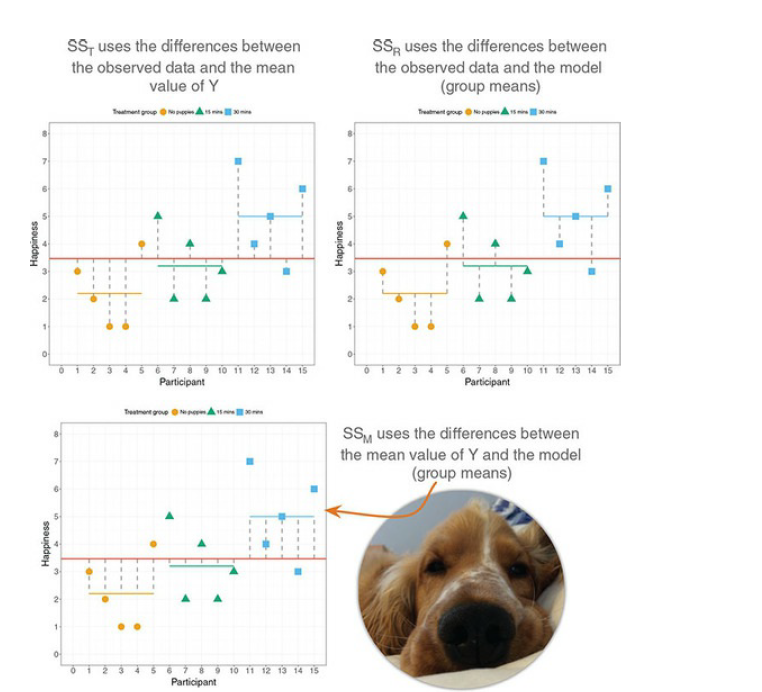
\includegraphics[width=1\textwidth,height=100mm]{Chapter 12 GLM 1 Comparing Several Independent Means ANOVA/sumofsquarederror.PNG}
	\caption{graphical representation of $SS_T$, $SS_R$,  $SS_M$. Experiment has 3 different groups, each with sample size of 5. Red line represent grand mean, shorter coloured lines represent group mean in the samples.}
\end{figure}

Equation of \textbf{$SS_M$}:
\begin{equation}
\text{SS}_M = \sum^k_{g=1} n_g(\bar{x}_g - \bar{x}_{grand})^2
\end{equation}

Equation is saying:
\begin{enumerate}
\item calculate the difference between the mean of each group ($\bar{x}_g$) and the grand mean ($\bar{x}_{grand}$).
\item Square each of the differences
\item Multiply each result by number of participants within the group ($n_g$)
\item Add the values for each group together
\end{enumerate}

For $SS_M$ the \textbf{degrees of freedom} ($df_M$) is the number of groups - 1, denoted by ($k-1$). 

\section{Residual sum of squares ($SS_R$)}
\textbf{Residual sum of squares} ($SS_R$) tells you how much variation cannot be explained by the model. This variation is caused by things we haven't measured such as measurement error, random noise and individual differences that may affect the DV other than our IV. 
Simplest way to calculate $SS_R$ is: 
\begin{center}
$SS_R = SS_T - SS_M$
\end{center}
However this provides little insight to what $SS_R$ represents.

We know that our model predicts the \textbf{mean of the group to which the person belongs}. Therefore, $SS_R$ is calculated by looking at the difference between the score obtained by the a person and the mean of the group to which the person belongs. In graphical terms, the dotted vertical lines in the figure represent difference. The distances between each data point and the group mean are squared and added together to give the residual sum of squares, $SS_R$:

\begin{equation}
SS_R = \sum^k_{g=1} \sum^n_{i=1} (x_{ig}-\bar{x}_g)^2
\end{equation}

We can also express $SS_R$ as:
\begin{equation}
SS_R = SS_{group 1} + SS_{group 2} + ... + SS_{group k}
\end{equation}
where k is the number of groups. 

Given that variance is the sum of squares divided by n -1, we can express $SS_R$ like this:
\begin{equation}
SS_R = \sum^k_{g=1} s^2_g (n_g - 1)
\end{equation}
This means that you multiply the variance for each group ($s^2_g$) by number of people in the group minus 1 ($n_g -1$, i.e. the $df_{within}$).

The degrees of freedom for $SS_R$ ($df_R$) is the total degrees of freedom minus the degrees of freedom for the model.
\begin{equation}
df_R = df_T - df_M
\end{equation}

This is equivalent to N - k, where N is total participants, and k is the number of groups. 

\section{Mean squares}
$SS_M$ tells you the total variation that the model explains (i.e. variation due to experimental manipulation), $SS_R$ tells you the total variation that is due to unmeasured factors. However, both SS are sum values,their size then depends on the number of scores. Furthermore $SS_M$ uses the sum of 3 values (group means) while $SS_R$ and $SS_R$ uses the sum of 15 values. We need to use MS instead in order to eliminate the discrepancies in size. 

However rather than dividing by the number of scores for each SS, we divide by the df as we are trying to extrapolate to a population and so some parameters within that population will be held constant

\begin{equation}
\begin{split}
MS_M & = \frac{SS_M}{df_M} \\
MS_R & = \frac{SS_R}{df_R} \\
\end{split}
\end{equation}

\section{F statistic}
F statistic is the measure of the ratio of variation explained by the model and the variation attributable to unsystematic factors. 
It is calculated by:
\begin{equation}
F = \frac{MS_M}{MS_R}
\end{equation}

If F is less than 1 it means that $MS_R$ is greater than $MS_M$ and that there is more unsystematic variance than systematic variance. This means that our experimental manipulation is unsuccessful and F will be non-significant.

\section{Interpreting F}
F is an \textbf{omnibus} test. A significant F tells us that the different groups are not equal but then, it does not tell you whether all of them are different or only some of them are different.

However if we want to see whether specific group means differ, we cannot just fit lots of model each of which compares only two means at a time; This is inflate the type 1 error rate. 

The reason why F-test is useful is that as a single test, it controls Type I error rate. Having established that overall group means differ (i.e. the outcome can be significantly predicted using the group means), we can use the parameters of the model ($b$-values) to tell us where the differences lie. 

\section{Assumptions when comparing means}
Given that we are still using a linear model, all assumptions that we have when doing normal hypothesis testing also applies. Normality is tested within groups, not across entire samples. 
\subsection{Homogeneity of variance}
We assume that variance of the outcome is steady as the predictor changes, (i.e. variances in the groups are equal). 
If group sizes are unequal, violations of the assumption of homogeneity of variance can have serious consequence. 
F test can be corrected to account for deviations from homogeneity. 
\begin{enumerate}
\item Brown-Forsythe F
\item Welsch's F
\end{enumerate}

\subsection{Brown-Forsythe F}
F is conservative when group sizes are unequal and the large groups have the biggest variance. If sample size is too large, it will inflate value of $SS_R$ as it is calculated by variance multiplied by sample size -1. If $SS_R$ is big, F will be smaller. 

Brown Forsythe got around this problem by weighting the group variances not by their sample size, but by the inverse of their sample size (they use $\frac{n}{N}$ which is the sample as the sample size as a proportion of the total sample size. This adjustment reduces the impact of large sample sizes with large variances.

\begin{equation}
\begin{split}
F_{BF} & = \frac{SS_M}{SS_{R_{BF}}}  =\frac{SS_M}{\sum s^2_k (1-\frac{n_k}{N})}  \\
& = \frac{SS_M}{s^2_{group1}(1-\frac{n_{group1}}{N}) + s^2_{group2}(1-\frac{n_{group2}}{N}) + s^2_{groupn}(1-\frac{n_{groupn}}{N})}
\end{split}
\end{equation}


\section{Is Anova Robust?}
Robust means that even if we break assumptions, the test will still be accurate.
Questions to ask:
\begin{enumerate}
\item Does F control the Type I error rate or is it significant even when there are no differences between means?
\item Does F have enough power to detect differences when they are there?
\end{enumerate}

Recent simulations shows that differences in skewness, non-normality and heteroscedasticity of variance interact in complicated ways that impact power. In the absence of normality, violations of homoscedasticity will affect F even when group sizes are equal. 

F can only be considered robust if \textbf{group distributions are identical}; e.g. all the groups if they are not normal, must be skewed in an identical way. 

\textbf{Violations of normality}: Heavy tailed distributions are problematic: if you set up a situation with power of 0.9 to detect an effect from a normal distribution and contaminate the distribution with 10\% scores from a normal distribution with a heavier tail, power drops to 0.28.  Heavy tailed distribution would need a greater sample size in order for central limit theorem to work (160 instead of usual 30).

\textbf{Violations of Assumptions of independence} is also very serious: if three groups of 10 observation per group are correlated at r = .5 , Type I error rate is 0.74 (when we thought it to be 0.05).

\section{What to do when assumptions are violated?}
If you routinely use Welch's F, then you no need to think about homogenity of variance, you can bootstrap parameter estimates which wont affect F itself and you know at least model parameters are robust.

If you can also use a robust test in all situation and not worry about the assumptions.

If you use the usual F statistic, at least conduct a sensitivity analysis, apply a robust test to check that your conclusion doesn't change. 

\section{Planned contrast (contrast coding)}
When we are using t test to check whether $b$ is significantly from 0 ($b$ is the differences between means), the trouble comes when we have 2 dummy variables and we need to do 2 t-tests, this will inflate the familywise error rate. 

Another problem is that dummy variables might not make all the comparisons we want to make. (in our example it doesnt compare 15 and 30 mins).

Solution is to use contrast coding rather than dummy coding. Contrast coding is a way of assigning weights to groups in dummy variables to carry out planned contrasts (known as planned comparisons). Weights are assigned in such a way that the contrasts are independent, which means Type I error rate is controlled. 

Another solution is to do a post hoc test: compare every mean group to all others (to conduct several overlapping tests using a t-statistic each time) but using a stricter acceptance criterion that keeps family wise error rate at .05. 

\section{Choosing which contrast to use}
In the puppy example, we may have 2 different hypothesis: 1) to test whether any puppy therapy would change happiness compared to control group. 2) Whether a 30 minute session could increase happiness more than a 15 minute one. 

To do a planned contrast, hypothesis must be derived before data are collected. F statistic is based on $SS_M$ and $SS_R$. Planned contrasts extend the logic by breakdown $SS_M$ into component parts. The exact contrast will depend on the hypothesis you want to test. 

\begin{figure}[h]
	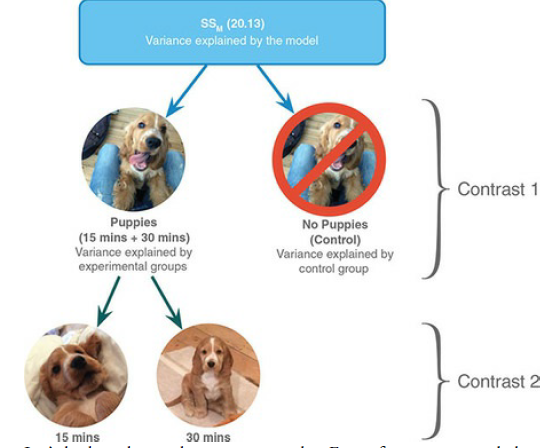
\includegraphics[width=0.5\textwidth,height=50mm]{Chapter 12 GLM 1 Comparing Several Independent Means ANOVA/plannedcontrast.PNG}
	\caption{graphical representation of $SS_T$, $SS_R$,  $SS_M$. $SS_M$ split into 2 more components: 15 mins and 30mins}
\end{figure}


Rules in designing planned contrasts:
\begin{enumerate}
\item \textbf{If you have a control group, this is because you want to compare it against any other groups}: Your first contrast will be the one that compares all the experimental groups with the control group. Once you done this first contrast, any remaining contrast will depend upon which groups you predict will differ (based on the theory you are testing). 
\item \textbf{Each contrast must compare only "two" chunks of variation}: Given that F is an omnibus test, we want to compare two chunks of variance only so that we know that the result represents a significance difference (or not) between the two portions of variation. If you follow the independents of contrast rule (rule 3), then you will always only compare two pieces of variance, then you should only end up with k - 1 contrasts (where k is the number of conditions you are comparing). 
\item \textbf{Once a group has been singled out in a contrast, it can't be used in another contrast}: we are breaking one chunk of variation into smaller independent chunks. The independence matters for controlling Type 1 error rate. Once a slice of variance has been split from a larger chunk, it cannot be attached to any other pieces of variance; it can only be further subdivided into smaller variance chunks. In our example given that contrast 1 compares control group with experimental group, it cannot be incorporated into contrast 2. 
\end{enumerate}


\begin{figure}[h]
	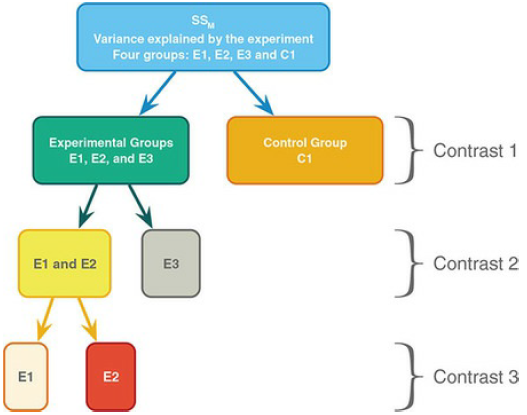
\includegraphics[width=0.5\textwidth,height=50mm]{Chapter 12 GLM 1 Comparing Several Independent Means ANOVA/plannedcontrast2.PNG}
	\caption{Planned contrast in a four group experiment using one control group}
\end{figure}

First contrast compare all the experimental groups with control group. Second contrast compares Experiment group 1 and 2 with Experimental group 3 (you can compare 1 and 3 with 2 as well, or 2 and 3 with 1). Final contrast compare the remaining chunk of variance not compared. 

In contrast, we are testing whether the group means are significantly differ from each other. If you are comparing two experimental group with one control. you are comparing the mean of the control group to the average mean of the 2 experimental group. All this comparisons is done using \emph{post hoc} tests.
\clearpage
\begin{figure}[h]
	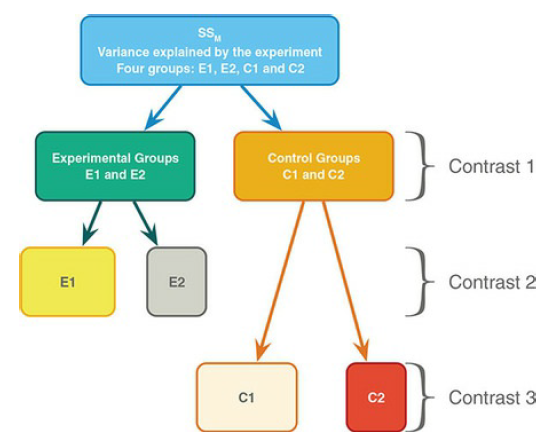
\includegraphics[width=0.5\textwidth,height=50mm]{Chapter 12 GLM 1 Comparing Several Independent Means ANOVA/plannedcontrast3.PNG}
	\caption{Planned contrast in a four group experiment using 2 experimental and 2 control group}
\end{figure}

For 2 control group is the same. You subdivide control group into smaller chunks and make sure that comparing contrasts are not repeated for the same chunk of variance. 

\section{Defining contrasts using weights}

\textbf{Weights} are the values assign to dummy variables usually 0 and 1. 

Rules of assigning values to contrasts:
\begin{itemize}
\item Rule 1: Choose sensible contrasts. Remember that you want to compare only two
chunks of variation and that if a group is singled out in one contrast, that group
should be excluded from any subsequent contrasts.

\item Rule 2: Groups coded with positive weights will be compared against groups coded
with negative weights. So, assign one chunk of variation positive weights and the
opposite chunk negative weights.
\item Rule 3: If you add up the weights for a given contrast the result should be zero.
\item Rule 4: If a group is not involved in a contrast, automatically assign it a weight of
zero, which will eliminate it from the contrast.
\item Rule 5: For a given contrast, the weights assigned to the group(s) in one chunk of
variation should be equal to the number of groups in the opposite chunk of variation.
\end{itemize}
\begin{figure}[h]
	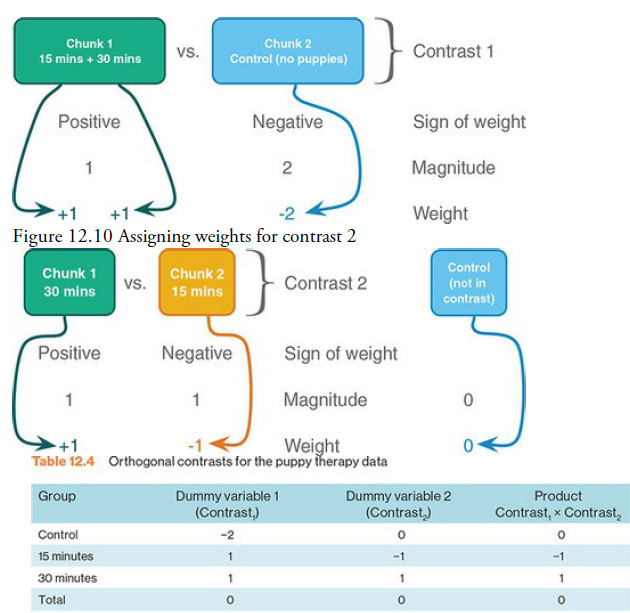
\includegraphics[width=1\textwidth,height=130mm]{Chapter 12 GLM 1 Comparing Several Independent Means ANOVA/orthogonalcontrast.PNG}
	\caption{Orthogonal contrast and its dummy coding. each dummy variable is one contrast. must ensure that the Final sum of (product of contrast 1 and contrast 2) = 0}
\end{figure}

It is important that the weights for a contrast sum to zero as you are comparing two unique chunks of variation, so that  t test can be used (which assumes independence).  products of contrast 1 and contrast 2 should also sum to 0. 

If contrasts are not indepedent, familywise rate will be infalted. However, if the products sum to zero then contrasts are independent or orthogonal. 
\clearpage
To put the dummy coding into a linear equation, it will be. 

\begin{equation}
\text{Happiness} = b_0 + b_1\text{Contrast}_{1i} + b_2\text{Contrast}{2i}
\end{equation}

If you substitute, $b$ with their corresponding dummy contrast code you will get. 

\begin{equation}
\begin{split}
b_0 & = \text{grand mean} = \frac{\bar{X}_{\text{30mins}} + \bar{X}_{\text{15 mins}} + \bar{X}_{\text{Control}}}{3} \\
b_1 & = \frac{1}{3}[(\frac{\bar{X}_{\text{30mins}} + \bar{X}_{\text{15 mins}}}{2}) - \bar{X}_{\text{Control}}] \\
b_2 & = \frac{\bar{X}_{\text{30mins}} - \bar{X}_{\text{15 mins}}}{2}
\end{split}
\end{equation}

\clearpage
\section{Built in Contrasts}

\begin{figure}[h]
	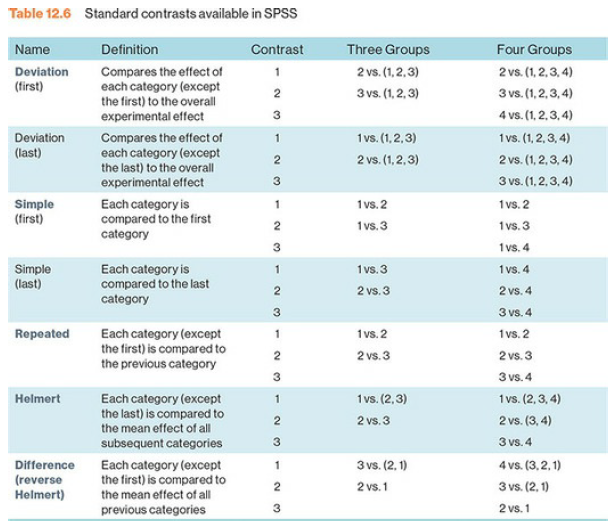
\includegraphics[width=1\textwidth,height=110mm]{Chapter 12 GLM 1 Comparing Several Independent Means ANOVA/builtincontrast.PNG}
	\caption{Different type of built in contrast in SPSS}
\end{figure}

Some of the contrast in SPSS are orthogonal (e.g. Helmert and difference contrasts) while others are non-orthogonal (deviation, simple and repeated)

\section{Polynomial contrasts: trend analysis}
Polynomial trend example: 
\begin{enumerate}
\item quadratic trend:  a drug enhances a performance on a task at first but drops performance as the dose increase. To find a quadratic trend, need at least 3 groups as 2 groups can only show linear trend. 
\item cubic trend: two changes in the direction of the trend: DV goes up down up across the various IV. 
\item quartic: 3 changes in direction.
\end{enumerate}

Contrasts for polynomial trends can be orthogonal.

\section{Post hoc procedures}
Post hoc tests consist of pairwise comparisons that are designed to compare all different combination of the treatment group. Taking every pair of groups and performing a separate test on each. However pairwise comparisons control the familywise error by correcting level of significance such that overall Type 1 error rate is $\alpha$. 

Most popular correction is called Bonferroni correction. 

For each post hoc tests ask the question:
\begin{enumerate}
\item Does the test control the Type I error rate?
\item Does the test control the Type II error rate?
\item is the test cobust?
\end{enumerate}

\subsection{Type I and Type II error rates for post hoc tests}

Always a trade off between Type 1 error rate and statistical power of a test.

If a test is conservative (Type I error will be small) then it is likely to lack statistical power (Type II error will be high). Important that multiple comparison procedures control the Type I error rate but without a substantial loss in power. 

\begin{itemize}
\item \textbf{Least-Significant Difference (LSD)} pairwise comparison makes no attempt to control Type I error and is equivalent to performing multiple tests on the data. Only difference is that LSD requires overall ANOVA to be significant.
\item \textbf{Studentized Newman-Keuls (SNK)} procedure is a liberal test but lacks control over the familywise error rate
\item \textbf{Bonferroni's} and \textbf{Tukey's} test both control Type I error rate very well but are conservative (lack statistical power). Bonferroni has more power when the number of comparison is small, Tukey is more powerful when testing large number of means. Tukey has greater power than \textbf{Dunn} and \textbf{Scheffe} tests.
\item The \textbf{Ryan, Einot, Gabriel, Welsch Q} procedure (REGWQ) has good power and tight control of Type I error rate. If you want to test all pairs of means, this procedure is the best. 
\end{itemize}

When there is equal sample sizes, and equal group variance, use REGWQ or Tukey. If want guaranteed control over Type I error, use Bonferroni.

\subsection{Are post hoc procedures robust?}
Most research on post hoc tests has looked at whetehr test performs well when group sizes are different, when population variances are different and when data is not normally distributed. Multiple comparison procedures perform relative well under small deviations of normality. But it performs badly when group sizes are unequal and variances are different. 

When sample sizes are different use: 
\begin {itemize}
\item \textbf{Hochberg's GT2} and 
\item \textbf{Gabriel's pairwise test} procedure 
\end{itemize} 
They are designed to cope with situations when sample sizes are different. Gabriels procedure is generally more powerful but but can be too liberal when sample size are too different.  Hochberg's GT2 is unreliable when population variances are different. 

When population variance differ use:
\begin{itemize}
\item Tamhane’s T2
\item Dunnett’s T3
\item Games–Howell 
\item Dunnett’s C. 
\end{itemize}